\chapter{基于雷尼散度的有辅助信息的随机块模型研究}
\label{chap:sbmsi}
\section{本章引言}
在本章中,我们首先介绍有辅助信息的随机块模型
的定义。
我们在前人研究的基础上,给出两社团情形下的精确恢复条件。
在精确恢复条件被保证的前提下,
我们将利用雷尼散度这一度量进一步研究
具有不同稀疏程度的模型的误差衰减率。
除此之外,我们将证明通过求解某半正定规划问题,可实现精确
恢复的要求,而该等价的优化问题可通过交替方向乘子法(ADMM)进行求解。

本章内容的具体安排如下:
在 \ref{sec:sbmsi_exact_recovery_condition} 节,我们给出了
带有辅助信息的随机块模型的精确恢复条件;
在 \ref{sec:sbmsi_error_decay_rate} 节,我们研究了算法的最优误差衰减速率,
在 \ref{sec:sdp_exact} 节,我们给出了一个能实现精确恢复的SDP算法,并通过实验
验证了其精确恢复效果。
第 \ref{sec:summary_sbmsi} 节对全章进行了总结。

\section{精确恢复条件}\label{sec:sbmsi_exact_recovery_condition}
\newacronym{acr:sbmsi}{SBMSI}{Stochastic Block Model with side information}
带有辅助信息的随机块模型(\gls{acr:sbmsi})
是 \ref{sec:sbm} 节介绍的
SSBM 模型的推广。为方便讨论又不失一般性,
这里我们在2个社团的随机块模型的
基础上引入辅助信息。
由定义 \ref{def:SSBM},当$k=2$时,
节点标签$X$满足$X_i \in \{\pm 1\}$
且 $\sum_{i=1}^n X_i = 0$。
除了图中边的集合
$\{Z_{i,j}\}_{1\le i<j\le n}$
和节点标签 $X$ 外,
第 $i$  个节点 ($1\leq i \leq n$) 
还含有 $m=\lceil \gamma \log n \rceil $ 个相关的数据样本 
$\{Y^{i}_j\}_{1\leq j \leq m}$。
这里,我们要求 $\gamma$ 是一个正整数。
若 $X_i=1$,
这些样本 i.i.d. 采样自分布 $P_0$,
若 $X_i=-1$,则采样自 $P_1$。
这里假设 $P_0, P_1$ 两个分布函数均为定义在字母集$\mathcal{Y}$上的离散分布。
注意到 给定 标签 $X_i$,
对于 $i\in [n]$,数据样本 $\{Y^{i}_j\}_{1\leq j \leq m}$ 与 $\{Z_{i,j}\}_{1\le i<j\le n}$ 独立。
 因此,在标签 $X$ 给定的情况下,
  $(\{Z_{i,j}\}_{1\le i<j\le n},\{Y^i_{j}\}_{1\le i\le n,1\le j\le m})$ 的联合分布为  
\begin{align}\label{eq:lh}
    &P(y=\{y^i_{j}\}_{1\le i\le n,1\le j\le m},z=\{z_{i,j}\}_{1\le i<j\le n}| (x_1,\ldots,x_n)) \nonumber\\
    &= \prod_{1\le i < j\le n}P(z_{i,j}|x_i,x_j)\prod_{i=1}^n \prod_{j=1}^m P(y^i_j|x_i), 
\end{align}
其中$\prod_{1\le i,j\le n}P(z_{i,j}|x_i,x_j)$ 可写成
式\eqref{eq:mle_sibm} 的形式。
对于$P(z_{i,j}|x_i,x_j)$,其具体定义为
\begin{equation*}
    P  (z_{i,j}=1|x_i,x_j) = \begin{cases}
        p & \text{if } x_i = x_j \\
        q & \text{if } x_i\ne x_j
    \end{cases},
\end{equation*}
并且
\begin{equation*}
    P(y^i_j|x_i) = \begin{cases}
        P_0(y^i_j) & x_i = 1 \\
        P_1(y^i_j) & x_i = -1
    \end{cases}
\end{equation*}
 $P(\{y^i_{j}\}_{1\le i\le n,1\le j\le m},\{z_{i,j}\}_{1\le i<j\le n}| x_1,\ldots,x_n)$ 
 的条件分布 依赖于
 $n,m,p, q, P_0$ 和 $P_1$ 这些参数,因此我们把 SBMSI 写成 $\SBMSI(n,m,p,q,P_0,P_1)$ 的形式。
 给定由 $\SBMSI(n,m,p,q,P_0,P_1)$ 生成的边$Z$和数据$Y$, 我们的目标是恢复 出$X$。
 
 在有辅助信息$Y$的条件下,
 我们仍使用能否精确恢复这一指标来衡量
 社团发现算法的准确性。
 与定义 \ref{def:SSBMR} 类似,
 若存在以$Z,Y$为输入变量的算法 $\hat{X}=\hat{X}(Z,Y)$
 使得当$n$增大时,
 错误概率
 $P_e:=P(\hat{Y} \neq Y)$ 趋向于 $0$,则称
 精确恢复可实现。

 文献\inlinecite{abbe2015community}中的3.2小节指出了一般随机块模型
 的精确恢复条件与多维泊松分布的关系。
在$k=2$的情形,我们要用到2维泊松分布,因此这里对其做一个简单的介绍。
有多种方式可推广一维的泊松分布,这里我们使用的是如下形式的二维泊松分布:

\begin{definition}
    称 $(X,Y)$ 服从参数为 $(\lambda, \mu)$ 的二维泊松分布,
    如果其概率质量函数为:
    \begin{equation}
        P(X=k, Y=j) = \frac{\lambda^k \mu^j}{k! j!}
        e^{-\lambda - \mu}, k,j=0,1,\dots
    \end{equation}
    记为 $(X,Y) \sim \Pois(\lambda, \mu)$。
\end{definition}

有了2维泊松分布的定义式,我们下面给出
SBMSI 模型精确恢复的条件:
\begin{theorem}\label{thm:Pe}
    定义$I_+$ 为联合分布 $\textrm{Pois}(\frac{a}{2},\frac{b}{2})\times \underbrace{P_0 \times \dots \times P_0}_{\gamma}$
    与 $\textrm{Pois}(\frac{b}{2}, \frac{a}{2})\times \underbrace{P_1 \times \dots \times P_1}_{\gamma}$ 
    之间的切尔诺夫信息。    
    对于 $\SBMSI(n,m=\lceil \gamma \log n \rceil, p=a\frac{\log n}{n},q=b\frac{\log n}{n},P_0,P_1)$,
    如果 $I_+>1$,则精确恢复可实现;
    如果 $I_+ < 1$,
    则错误概率 $P_e$ 趋近于 $1$,精确恢复不可实现。
\end{theorem}

定理 \ref{thm:Pe} 类似于文献 \inlinecite{abbe17sideinfo} 中定理4的结论,
但这里我们允许采样数量 $m$ 为
$\lceil \log n \rceil $ 的整数倍,同时
限制了类别数为2的条件,而 文献 \inlinecite{abbe17sideinfo} 的定理4
中始终取$\gamma=1$。

对于一般的情形,SBMSI 模型精确恢复的 临界值 $I_+$ 并没有
显示表达式,但我们可以从切尔诺夫信息的定义出发得到 $I_+$ 的简化表达式,
该表达式由下述引理 \ref{lem:I_plus_expression} 给出,
其更容易计算,且在后面定理 \ref{thm:sdp} 的证明中也会用到。

\begin{lemma}\label{lem:I_plus_expression}
\begin{align}\label{equation:I+}
    I_+ &=\frac{\lambda^* }{2} (a^{1-\lambda^* }b^{\lambda^* } -
    b^{1-\lambda^* }a^{\lambda^* })\log\frac{b}{a}+\frac{a+b}{2}\notag \\
    &-\frac{1}{2}(a^{1-\lambda^*}b^{\lambda^*} +
    b^{1-\lambda^* }a^{\lambda^* })+\gamma D(P_{\lambda^* }||P_0) 
	\end{align}
	其中
	\begin{equation}\label{eq:lambda}
    \lambda^* = \arg\min_{\lambda} \left[a^{1-\lambda}b^{\lambda} +
    b^{1-\lambda}a^{\lambda} + 2\gamma \log
    \left(\sum_{x\in \mathcal{X}}P^{1-\lambda}_0(x) P^{\lambda}_1(x)
    \right)
    \right]
\end{equation}
而 $P_{\lambda}$ 类似式\eqref{eq:P_lambda_x},为
\begin{equation}\label{eq:P_lambda_0_1}
    P_{\lambda}(x) = \frac{P_0^{1-\lambda}(x) P_1^{\lambda} (x)}
    {\sum_{x \in \mathcal{X}}P_0^{1-\lambda}(x) P_1^{\lambda} (x)}        
\end{equation}

\end{lemma}


%\section{引理 \ref{lem:I_plus_expression} 的证明}
在证明引理
 \ref{lem:I_plus_expression}   之前,
我们先列举泊松分布的一个重要的性质。
\begin{lemma}\label{lem:poisson_property}
假设 $P_0 \sim \Pois(c)$, $P_1 \sim \Pois(d)$,
且 $P_{\lambda}$ 由 式\eqref{eq:P_lambda_0_1}
给出。

则我们有
\begin{enumerate}
    \item $P_{\lambda} \sim \Pois(c^{1-\lambda} d^{\lambda})$
    \item $D(P_{\lambda}||P_0) = 
    \lambda c^{1-\lambda}d^{\lambda}\log(\frac{d}{c}) + c-c^{1-\lambda}d^{\lambda}$
    \item $D(P_{\lambda}||P_1) = (1-\lambda)
    c^{1-\lambda}d^{\lambda}\log(\frac{c}{d})
    + d-c^{1-\lambda}d^{\lambda}$
\end{enumerate}
\end{lemma}
上面的第2、3条性质可由两个泊松分布的KL散度
公式导出。
\begin{proof}[引理 \ref{lem:I_plus_expression} 的证明]
由 切尔诺夫信息的定义式 \eqref{eq:D_star_lambda_star} 
可得:
$$
I_+ = D(\hat{P}_{\lambda^*} || \Pois(\frac{a}{2}))
+ D(\hat{P}_{1-\lambda^*} || \Pois(\frac{b}{2}))
+ \gamma D(P_{\lambda^*} || P_0)
$$
其中 $\hat{P}_{\lambda^*}$由
引理 \ref{lem:poisson_property} 第一条
性质确定,而我们取$c=\frac{a}{2}, d=\frac{b}{2}$。
继续应用引理 \ref{lem:poisson_property} 第2-3条性质可得
\begin{align*}
    I_+ &= \left[\lambda^* c^{1-\lambda^*}d^{\lambda^*}
    \log(\frac{d}{c})+ c-c^{1-\lambda^*}d^{\lambda^*}
    \right] \\
&+ \left[\lambda^* c^{\lambda^*}d^{1-\lambda^*}\log(\frac{c}{d})
+ d - c^{\lambda^*}d^{1-\lambda^*}\right]
+ \gamma D(P_{\lambda^*} || P_0)
\end{align*}
即得式\eqref{equation:I+}。
$\lambda^*$ 可由式\eqref{eq:C_P_1_P_2_another} 
进行计算。目标函数为:
\begin{align*}
&\log\left(\sum_{k=0}^{+\infty} \left(\frac{c^k\exp(-c)}{k!}
\right)^{1-\lambda}
\left(\frac{d^k\exp(-d)}{k!} \right)^{\lambda}
\right) \\
& + \log\left(\sum_{k=0}^{+\infty} \left(\frac{c^k\exp(-c)}{k!}
\right)^{\lambda}
\left(\frac{d^k\exp(-d)}{k!} \right)^{1-\lambda}
\right)+
\gamma\log(\sum_{x\in \mathcal{X}}P^{1-\lambda}_0(x) P^{\lambda}_1(x)
)\\
& = c^{1-\lambda} d^{\lambda} 
+ d^{\lambda} c^{1-\lambda} -c -d +
\gamma\log \left(\sum_{x\in \mathcal{X}}P^{1-\lambda}_0(x) P^{\lambda}_1(x)
\right)
\end{align*}
极小化上式即等价于式\eqref{eq:lambda}。
\end{proof}

\begin{remark}
当 $\gamma=0$ 时,由式\eqref{eq:lambda} 可得 $\lambda^*=\frac{1}{2}$,
则 $I_+=\frac{1}{2}(\sqrt{a}-\sqrt{b})^2$。由 式 \eqref{eq:renyi_d12_ab},
$I_+$ 也可写成雷尼散度的形式。
进一步地,由定理 \ref{thm:Pe},$\sqrt{a}-\sqrt{b} > \sqrt{2}$
时可精确恢复。定理 \ref{thm:Pe} 退化到
定理 \ref{thm:sbm2_phase_transition}。
\end{remark}

\section{误差衰减速率}\label{sec:sbmsi_error_decay_rate}
在 \ref{sec:sbmsi_exact_recovery_condition} 节的基础上,
我们讨论一种更强的要求,即恢复算法将SSBM各社团大小相等的条件考虑在内。
类似定理 \ref{thm:error_rate},
在这种情况下,利用带约束的最大似然估计,我们可以得到恢复算法更快的误差衰减速率。
%{eq:mle_sibm}

具体而言,在式\eqref{eq:lh}中极小化$x$
可得到如下的优化问题:
\begin{align}
    \hat{X} &= \arg\max_x\ P(y,z|X=x) \notag \\
    \textrm{s.t.} \ & x_i \in \{\pm 1\}, \sum_{i=1}^n x_i=0 \label{eq:mle}
\end{align}
类似式\eqref{eq:hatX_double_prime},
由式\eqref{eq:mle}给出的估计量 $\hat{X}$,
是在有约束的参数空间内的最大似然估计量。
如果我们修改定义 \ref{def:SSBM} 中真实标签$X$的生成方式,
使得$X_1, \dots, X_n$ i.i.d. $\sim \Bern(\frac{1}{2})$,
则应该使用不带约束的 ML 估计量进行社团发现。

根据 SBMSI 中的 随机块模型参数 $p,q$ 随 $n$的变化规律,我们下面分两种情况讨论。
\subsection{稀疏的 SSBM }
\newglossaryentry{not:big_o}
{
  type=notation,
  name={$f(n)=O(g(n))$},
  description={大O符号,表示存在常数$C$和正整数$N$,使得$f(n)\leq C g(n)$ 对于$n\geq N$均成立}
}
当SSBM 的 $p,q$ 参数以 $O(\frac{ \log n}{n})$
的速率衰减时,我们有如下定理:
\begin{theorem}\label{thm:Pe_new}
    令
    $\gamma = \frac{ m}{\log n}$
    为一常数。
    若
    $p = \frac{a \log n }{n} $ 且 $q = 
    \frac{b \log n } {n}$,使用最大似然估计量 \eqref{eq:mle}
    进行社团发现,
    若
    \begin{equation}\label{eq:positive_condition_new}
    \gamma D_{1/2}(P_0||P_1) +
     (\sqrt{a} - \sqrt{b})^2-2 > 0
    \end{equation}
    则精确恢复的误差上界为:
    \begin{equation}\label{eq:PeMain}
    P_e \leq \left(\frac{1}{4}+o(1) \right) n^{-\left(\gamma D_{1/2}(P_0||P_1) + (\sqrt{a} - \sqrt{b})^2-2 + o(1)\right) }
    \end{equation}
    如果下述条件满足,
    \begin{align}
    (\sqrt{a}-\sqrt{b})^2-2 
    > 3a^{1/3}b^{1/3}(a^{1/6}-b^{1/6})^2\label{eq:oneC}
    \end{align}
    则精确恢复的误差下界为:
    \begin{equation}\label{eq:PeMainL}
    P_e \geq \left(\frac{1}{4}+o(1) \right) n^{-\left(\gamma D_{1/2}(P_0||P_1) + (\sqrt{a} - \sqrt{b})^2-2 + o(1)\right)}
    \end{equation}
\end{theorem}

由定理 \ref{thm:Pe_new} 可看出,
误差界的幂次有两项组成,
一项 $\gamma D_{1/2}(P_0||P_1) $ 
和辅助信息有关,表示成$P_0$和$P_1$的雷尼散度(在式\eqref{eq:renyi_divergence}
中定义)
,另一项 $ (\sqrt{a} - \sqrt{b})^2-2 $
和 SSBM 的精确恢复条件有关,根据
式\eqref{eq:renyi_d12_ab},也可表示成雷尼散度的形式。

定理 \ref{thm:Pe_new} 告诉我们
辅助信息  $Y$  增大了 误差 $P_e$ 的衰减速率,
增大的程度可用雷尼散度表示的信息量
$\gamma D_{1/2}(P_0||P_1)$ 
来刻画。
若额外的参数条件 \eqref{eq:oneC} 成立,
可推出 式\eqref{eq:positive_condition_new} 也成立,
此时
误差衰减速率为:
$$
-\lim_{n\to \infty} \frac{\log P_e}{\log n}
= \gamma D_{1/2}(P_0||P_1) + (\sqrt{a} - \sqrt{b})^2-2
$$
此外,当 $P_0=P_1$ 时,
定理 \ref{thm:Pe_new} 给出了用带约束的最大似然算法
对SSBM 做社团发现
的误差衰减速率,总结为如下推论:
\begin{corollary}\label{cor:sbm}
考虑
$\SSBM(n,\frac{a\log n}{n}, \frac{b \log n}{n}, 2)$,
对于式\eqref{eq:mle}中的ML算法, 
若 条件 \eqref{eq:oneC} 成立,
则错误概率 $P_e$ 满足
\begin{equation}\label{eq:cor}
\lim_{n\to \infty} \frac{\log P_e}{\log n} =2-(\sqrt{a} - \sqrt{b})^2
\end{equation}

\end{corollary}
相比于定理 \ref{thm:error_rate} 中的第2条,
这里我们推导出了误差下界的表达式 \eqref{eq:PeMainL},
因而得到了紧的误差率 \eqref{eq:cor}。

下面我们讨论本节的误差衰减速率项
$\gamma D_{1/2}(P_0||P_1) +
(\sqrt{a} - \sqrt{b})^2$与上一节
精确恢复条件中的切尔诺夫信息量 $I^+$ 的关系。
我们有如下定理
\begin{theorem}\label{thm:I_plus_relation}
    设$I_+$ 在 式 \eqref{equation:I+}
    中定义,则
    \begin{equation}
        I_+ \geq \frac{1}{2}
        (\sqrt{a} - \sqrt{b})^2 +
        \frac{\gamma}{2} D_{1/2}(P_0||P_1)
    \end{equation}
\end{theorem}
	由定理 \ref{thm:I_plus_relation} 
    可知,随着  $\gamma$ 的增大, 即每个节点辅助采样数量的增多, $I_+$
    的下界增大。因此,更多的样本有助于满足精确恢复的条件 $I_+>1$。 

\subsection{稠密的 SSBM}
当 SSBM 的 $p,q$ 参数是常数时,我们有如下定理:
\begin{theorem}\label{thm:constant}
	令 $\gamma = \frac{m}{n}$ 为一常数。
    若 $p,q$ 为常数,使用最大似然估计量 \eqref{eq:mle}
    进行社团发现,
	精确恢复的误差指数
    为
    \newglossaryentry{not:bern}
{
  type=notation,
  name={$\Bern(p)$},
  description={参数为$p$的伯努利分布}
}
	\begin{equation}\label{eq:dense_error_exponent}
	-\lim_{n\to \infty} \frac{1}{n}\log P_e = 
     \gamma D_{1/2}(P_0 || P_1) + D_{1/2}(\Bern(p)||\Bern(q))
	\end{equation} 
\end{theorem}

由定理 \ref{thm:constant} 可知,精确恢复误差
随着$n$的增大
指数衰减。
当 $\gamma=0$ 时,定理 \ref{thm:constant} 指出
$D_{1/2}(\Bern(p)||\Bern(q))$
是精确恢复的误差指数。
因为
几乎完全恢复与精确恢复相差一个$n$的数量级,
$D_{1/2}(\Bern(p)||\Bern(q))$ 也是几乎完全恢复的误差指数
\cite{zhang2016}。
除此之外, 假设 $\gamma$ 为整数,
误差指数可视为 
联合分布
$\underbrace{P_0\times \dots \times P_0}_{\gamma} \times \Bern(p)$
和 $\underbrace{P_1\times \dots \times P_1}_{\gamma} \times \Bern(q)$
之间的雷尼散度。
由独立性条件,
我们可以把这一散度分解成如\eqref{eq:dense_error_exponent}
所示的两项求和的形式。
进一步地, 定理 \ref{thm:constant} 
的结果要求
$m$ 和 $n$ 量阶相同。
当 $m=o(n)$ 时,
图中边的信息占主导
地位;
而当 $m=\omega(n)$时,
每个节点的辅助信息占
主导地位,此时所研究的问题变成$n$个独立的假设检验问题。
\newglossaryentry{not:small_omega}
{
  type=notation,
  name={$f(n)=\omega(g(n))$},
  description={$\lim_{n\to \infty} \frac{f(n)}{g(n)} = +\infty$}
}

\section{实现精确恢复的SDP算法}\label{sec:sdp_exact}
\subsection{算法描述}
本节我们给出实现关于SBMSI 精确恢复的SDP算法。

%给定节点标签$X$,
%令 $S_1(X)$ 和 $S_2(X)$ 分别表示 标签为1和-1的节点集。
可以验证, 在 $X\in\{\pm 1\}^n$ 的取值范围内
极大化 关于
$(Y,Z)$ 的对数似然函数 式 \eqref{eq:lh} 等价于求解下面的优化问题
\begin{align}
    \max_{v}\, & h^T v + \frac{1}{4}v^T B v \notag \\
    \textrm{s.t. }\, & \mathbf{1}_n^T v = 0 \text{ 且 } v_i \in \{\pm 1 \} \label{eq:matrix_mle}
\end{align}
其中 $h$ 是 $n$ 长的向量,第 $i$ 个元素为$h_i = \frac{1}{\log \frac{a}{b}}\sum_{j=1}^m \log \frac{P_0(y^i_{j})}{P_1(y^i_{j})}, i\in [n]$,
而  $n\times n $ 的矩阵 $B$ 在 式\eqref{eq:def_B_sdp} 中定义。

令 $x^*$ 是 \eqref{eq:matrix_mle} 的最优值,
且 $V^*=(1,x^*)(1,x^*)^T$, 
其中 $(1,x^*)$ 是一个
将 $1$ 和 $x^*$ 连接起来的
$(n+1)$ 维的向量。
	则 式\eqref{eq:matrix_mle} 中目标函数的
    最优值等于 $\frac{1}{2} \langle \widetilde{B}, V^* \rangle$, 其中
	\begin{equation}\label{eq:B_lambda_def}
		\widetilde{B} = \begin{pmatrix} 0 & h^T  \\ h  & \frac{1}{2}B \end{pmatrix} 
	\end{equation}
	是一个$(n+1)\times(n+1)$的矩阵。我们将证明 $V^*$ 是如下问题的唯一最优解:
	\begin{align}
		\max_V\,& \langle \widetilde{B}, V \rangle  \notag\\
		\textrm{ s.t. }\, V_{ii} &= 1, \notag\\
		V &\succeq 0, \notag\\
\sum_{j=2}^{n+1} (V_{ij} + V_{ji})& = 0,~\forall\, i\in\{1,\ldots,n+1\} 
\label{eq:sdp}
	\end{align}
	注意到在 式\eqref{eq:sdp} 的最后一行
    我们用了 $n+1$ 个约束条件 来描述标签 平衡的条件。
    这些约束条件在证明$V^*$是式\eqref{eq:sdp}唯一的最优解时起到关键作用。
    该结论可总结为下述定理:

	\begin{theorem}\label{thm:sdp}
        设 $\hat{V}$ 是优化问题 \eqref{eq:sdp} 的解,
        $x^*$ 是真实的标签向量。
		若 $I_+ > 1$, 则
        $\lim_{n\to\infty} P(\hat{V}=V^*)=1$,其中
		$V^*=(1,x^*)(1,x^*)^T$。
	\end{theorem}
    该定理表明,只要满足恢复条件$I^+>1$,我们的SDP松弛方法可以高概率地实现社团结构的精确恢复。


\subsection{算法实现}\label{sec:sdp_admm}
虽然半正定规划问题\eqref{eq:sdp}可以使用一般的SDP优化工具包进行,但针对其特殊形式,
我们可以提前计算出投影矩阵,
从而实现算法加速。
这里我们借鉴文献 \inlinecite{amini2018semidefinite} 中针对无辅助信息设计的SDP-1的算法,
给出基于ADMM方法求解优化问题\eqref{eq:sdp}的算法实现。
为方便讨论,本节假设所有的矩阵都是 $n$维的,而式 \eqref{eq:sdp} 中矩阵的维数是$n+1$,只需作整体替换即可。

求解形如 式\eqref{eq:sdp} 的SDP优化问题可通过如下迭代进行,各矩阵的初始值$X^{(0)},Z^{(0)},U^{(0)}$可取为零矩阵。
\begin{align}
    X^{(k+1)} &= \Pi_A(Z^{(k)} - U^{(k)} + \frac{1}{\rho}B)\label{eq:admm} \\
    Z^{(k+1)} &= \Pi_{S_+^n}(X^{(k+1)} + U^{(k)}) \\
    U^{(k+1)} &= U^{(k)} + (X^{(k+1)} - Z^{(k+1)}) 
    \end{align}
其中 $\rho>0$ 是 惩罚参数,$\Pi_{S_+^n}$ 表示在半正定锥上的投影。
实际操作中先将输入矩阵 做特征值分解 $X=P\Lambda P^{-1}$,
再将负的特征值改为零即得投影矩阵$\Pi_{S_+^n}(X)=P\frac{|\Lambda| + \Lambda}{2}P^{-1}$。

$\Pi_A$也是矩阵投影算子,是把一个矩阵投影到$L(X) = b$这个空间内,
其中 $b=(0, -2 \mathbf{1}_{n-1}, \mathbf{1}_{n}) \in \mathbb{R}^{2n}$,
而
$L$ 是一个从 $\mathbb{R}^{n \times n} $ 到 $\mathbb{R}^{2n}$ 的线性映射。
$L$ 的精确定义需要引入矩阵$H_i$ 和 $F_i$,$i\in [n]$。
$H_1$ 是一个第一行和第一列非对角线上元素为1,其余位置为0的对称矩阵。
$H_i$ 是第$i$行和第$i$列非对角线上元素($H_{1i}$ 和 $H_{i1}$除外)为1,其余位置为0的对称矩阵。
$F_i$ 仅在  位置$(i,i)$上取 1,其余位置为0。
有了$H_i$ 和 $F_i$,对于 $i \in [n]$,
$[L(X)]_i = \langle X,H_i \rangle$ 且 $[L(X)]_{i+n} = \langle X,F_i \rangle$。

类似 $\Pi_{S_+^n}$, 我们可以通过矩阵运算来刻画投影算子 $\Pi_{A}$。 
$L$ 可视为一个 $2n \times n^2$ 的矩阵,
则矩阵 $Y$ 在 $L(X)=b$ 空间内的投影为
\begin{align}\label{eq:proj:L:Y}
\Pi_{A}(Y) := Y - L^* (L L^*)^{-1}[ L(Y) - b] 
\end{align}
其中 $L^*$  是 $L$ 的转置,设 $(\mu,\nu)$ 是一个$\mathbb{R}^{2n}$ 维的向量,
则我们有 $L^*((\mu,\nu)) = \sum_{i=1}^n \mu_i H_i + \sum_{i=1}^n \nu_i F_i$。
设 $(\mu',\nu')=LL^*((\mu,\nu))$。
则$\mu'_j = \sum_{i=1}^n \langle H_i, H_j \rangle \mu_i
=(2n-1)\mu'_j$,
$\nu'=\nu$。
因此 $L L^*$ 是一个 $2n\times 2n$的块对角矩阵 
$LL^*=\diag\{2(n-1), 2[(n-3)I_{n-1}+J_{n-1}],I_n\} $。
取矩阵$L L^*$的逆得
\begin{align*}
(LL^*)^{-1} = \diag\Big(\frac{1}{2n-2},\frac{1}{2(n-3)} 
\big[ I_{n-1} - \frac{J_{n-1}}{2n-4} \big],\; I_n \Big)
\end{align*}
于是我们给出了 投影算子 $\Pi_{A} $ 
的计算方法。

基于以上方法,我们开展了SDP算法对SBMSI模型精确恢复的仿真实验。
图 \ref{fig:my_label} 展示了 SDP算法
针对 带有辅助信息的随机块模型 实现精确恢复的成功率。
成功率是指 对每一组参数的若干次重复实验中,我们计算算法
实现精确恢复的比率。
我们固定 $n=300$, 对每一组参数$(a,b)$,重复次数是 20。
每个节点的辅助采样数量为 $m=10$,
$P_0,P_1$ 两个分布分别为 $\Bern(0.2)$ 和 $\Bern(0.8)$。
红线对应着有辅助信息的分界线 $I_+ = 1$。
由图可见,白色区域与灰色区域的分界线与红线 $I_+ = 1$ 大致对应,
从而验证了定理 \ref{thm:sdp} 中的结论。
另外在图中我们还画出了没有辅助信息时精确恢复的分界线,即蓝色的 
$\sqrt{a}-\sqrt{b}=\sqrt{2}$,取式\eqref{eq:cor}
的右端项为零即可得到。
将两条分界线进行对比可以看出辅助信息使得满足精确恢复的参数$(a,b)$的
组合更多了,降低了精确恢复的难度。

\begin{figure}[!ht]
    \centering
    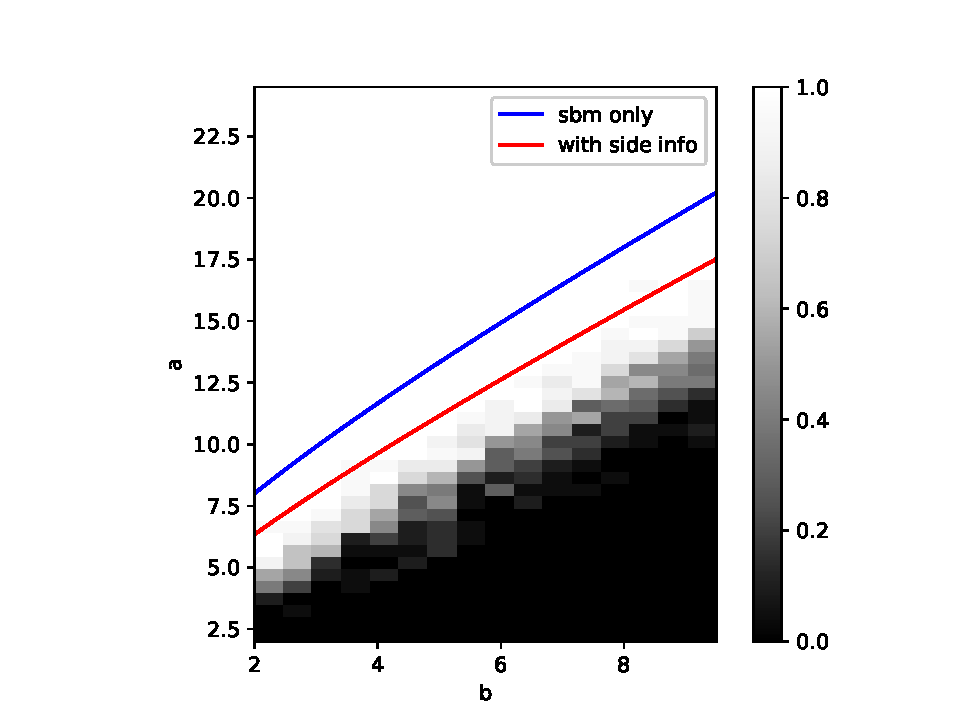
\includegraphics[width=0.8\textwidth]{new_results.pdf}
    \caption{有(无)辅助信息的分界线与SDP算法恢复性能的比较}
    \label{fig:my_label}
\end{figure}

\chapter{第 \ref{chap:sbmsi} 章补充内容}
		
\section{引理\ref{lem:I_plus_expression} 的证明}
在证明引理
\ref{lem:I_plus_expression}  之前,
我们先列举泊松分布的一个重要的性质。
\begin{lemma}\label{lem:poisson_property}
假设 $P_0 \sim \Pois(c)$, $P_1 \sim \Pois(d)$.
且 $P_{\lambda}$ 由 式\eqref{eq:P_lambda_0_1}
给出。

则我们有
\begin{enumerate}
    \item $P_{\lambda} \sim \Pois(c^{1-\lambda} d^{\lambda})$
    \item $D(P_{\lambda}||P_0) = 
    \lambda c^{1-\lambda}d^{\lambda}\log(\frac{d}{c}) + c-c^{1-\lambda}d^{\lambda}$
    \item $D(P_{\lambda}||P_1) = (1-\lambda)
    c^{1-\lambda}d^{\lambda}\log(\frac{c}{d})
    + d-c^{1-\lambda}d^{\lambda}$
\end{enumerate}
\end{lemma}
上面的第2、3条性质可由两个泊松分布的KL散度
公式导出。
\begin{proof}[引理\ref{lem:I_plus_expression} 的证明]
由 切尔诺夫信息的定义 \eqref{eq:D_star_lambda_star} 式
可得:
$$
I_+ = D(\hat{P}_{\lambda^*} || \Pois(\frac{a}{2}))
+ D(\hat{P}_{1-\lambda^*} || \Pois(\frac{b}{2}))
+ \gamma D(P_{\lambda^*} || P_0)
$$
其中 $\hat{P}_{\lambda^*}$由引理\ref{lem:poisson_property}
第一条性质确定,而我们取$c=\frac{a}{2}, d=\frac{b}{2}$。
继续应用引理\ref{lem:poisson_property}第2、3条性质可得
\begin{align*}
    I_+ = \left[\lambda^* c^{1-\lambda^*}d^{\lambda^*}
    \log(\frac{d}{c})+ c-c^{1-\lambda^*}d^{\lambda^*}
    \right]
+ \left[\lambda^* c^{\lambda^*}d^{1-\lambda^*}\log(\frac{c}{d})
+ d - c^{\lambda^*}d^{1-\lambda^*}\right]
+ \gamma D(P_{\lambda^*} || P_0)
\end{align*}
即\eqref{equation:I+} 式。
$\lambda^*$ 可由\eqref{eq:C_P_1_P_2_another} 式
进行计算。目标函数为:
\begin{align*}
&\log\left(\sum_{k=0}^{+\infty} \left(\frac{c^k\exp(-c)}{k!}
\right)^{1-\lambda}
\left(\frac{d^k\exp(-d)}{k!} \right)^{\lambda}
\right) \\
& + \log\left(\sum_{k=0}^{+\infty} \left(\frac{c^k\exp(-c)}{k!}
\right)^{\lambda}
\left(\frac{d^k\exp(-d)}{k!} \right)^{1-\lambda}
\right)+
\gamma\log(\sum_{x\in \mathcal{X}}P^{1-\lambda}_0(x) P^{\lambda}_1(x)
)\\
& = c^{1-\lambda} d^{\lambda} 
+ d^{\lambda} c^{1-\lambda} -c -d +
\gamma\log(\sum_{x\in \mathcal{X}}P^{1-\lambda}_0(x) P^{\lambda}_1(x)
)
\end{align*}
极小化上式即等价于\eqref{eq:lambda}式。
\end{proof}
\section{定理 \ref{thm:I_plus_relation} 的证明}
	\begin{lemma}\label{lem:p0p12}
        设 $P_{\widetilde{Y}}$ 是定义在字母集
        $\mathcal{Y}$ 上的分布函数。
		对于 $\SBMSI(n,m,p,q,P_0,P_1)$,定义
        $I_1, I_2$ 如下
		\begin{align}
			I_1 &=\min_{P_{\widetilde{Y}}} \gamma D(P_{\widetilde{Y}}|| P_0)+ \frac{1}{2} g(a,b, 2\epsilon),
            \text{ 其中}\nonumber\\
			\epsilon &= \gamma \frac{D(P_{\widetilde{Y}} || P_1) - D(P_{\widetilde{Y}} || P_0) }{\log \frac{a}{b}}\label{eq:I1}
		\end{align}
        函数 $g(a,b,\epsilon)$ 在式 \eqref{equation:g}中定义,而 $I_2$ 的定义通过交换 $P_0, P_1$ 的位置得到:
		\begin{align}
			I_2 & = \min_{P_{\widetilde{Y}}} \gamma D(P_{\widetilde{Y}}|| P_1)+ \frac{1}{2} g(a,b, 2\epsilon),
            \text{ 其中}\nonumber\\
			\epsilon &= \gamma \frac{D(P_{\widetilde{Y}} || P_0) - D(P_{\widetilde{Y}} || P_1) }{\log \frac{a}{b}}
            \label{eq:I2}
		\end{align}
 		则我们有 $I_1=I_2=I_+$. 
    \end{lemma}
    \begin{proof}
        我们只需证明 $I_1=I_+$ 成立即可。
另一半 $I_2=I_+$ 可由 $I_+$ 的定义对称性导出。

我们用 拉格朗日乘子法 来求解 \eqref{eq:I1}。
令
\begin{align*}
L(P_{\widetilde{Y}},\epsilon, \lambda)
=\gamma D(P_{\widetilde{Y}}|| P_0)+
\frac{1}{2} g(a,b, 2\epsilon)
- \lambda(\epsilon \log\frac{a}{b}-\gamma
D(P_{\widetilde{Y}} || P_1) + \gamma D(P_{\widetilde{Y}} || P_0))
\end{align*}
对于给定的 $\epsilon$,极小化 $L(P_{\widetilde{Y}},\epsilon, \lambda)$
相当于极小化
$(1-\lambda)D(P_{\widetilde{Y}} || P_0) +
\lambda D(P_{\widetilde{Y}} || P_1) $。通过类似
\citet{cover1999elements} 中 式(11.199) 中求导的方式,
我们得到 $P_{\widetilde{Y}}(y) = P_{\lambda}(y)$,
其中 $P_{\lambda}(y)$ 定义见式\eqref{eq:P_lambda_0_1}。
另一方面,由 $\frac{\partial L(P_{\widetilde{Y}},\epsilon, \lambda)}{\partial \epsilon}=0$
并将 式\eqref{eq:P_lambda_0_1}
代入到 式\eqref{eq:I1}, 我们得到
\begin{align*}
    \lambda \log \frac{a}{b}
    & = \log \frac{\epsilon + \sqrt{\epsilon^2+ab}}{b} \\
    \epsilon \log \frac{a}{b}
    & = \gamma\frac{\sum_{Y \in \mathcal{Y}}P_0^{1-\lambda}(y) P_1^{\lambda} (y)
    \log \frac{P_0(y)}{P_1(y)}}{\sum_{y \in \mathcal{Y}}
    P_0^{1-\lambda}(y) P_1^{\lambda} (y)}
\end{align*}
上述两式消掉 $\epsilon$ 后,我们可以得到关于
$\lambda$ 的方程:
\begin{align*}
    \frac{\log\frac{a}{b}}{2}
    (a^{\lambda} b^{1-\lambda}
    -a^{1-\lambda} b^{\lambda})
    + \gamma \frac{\sum_{y \in \mathcal{Y}}
    P_0^{1-\lambda}(y) P_1^{\lambda}(y)
    \log \frac{P_1(y)}{P_0(y)}}
    {\sum_{y \in \mathcal{Y}}P_0^{1-\lambda}(y)
    P_1^{\lambda} (y)}
    =0
\end{align*}
上式恰等价于 \eqref{eq:lambda} 式中目标函数对 $\lambda$求导后整个式子等于零。
因此$P_{\widetilde{Y}}=P_{\lambda^*}(\lambda)$。
代入$I_1$ 的表达式中化简后我们可得
$I_1 = I_+$。
\end{proof}
\begin{proof}[定理 \ref{thm:I_plus_relation} 的证明]
    由引理 \ref{lem:p0p12},
    我们只需证明 $I_1 \geq \frac{1}{2}[\gamma D_{1/2}(P_0||P_1)
    + (\sqrt{a} - \sqrt{b})^2]$。
    由于定义在 式\eqref{equation:g} 中的 $g(a,b,\epsilon)$ 是关于 $\epsilon$
    的凸函数,则我们有
    \begin{equation}\label{eq:g_linear}
            g(a,b,\epsilon) \geq g(a,b,0) + g'(a,b,0)\epsilon = (\sqrt{a} - \sqrt{b})^2 + \frac{\epsilon}{2}\log \frac{a}{b}. 
        \end{equation}
        则由引理 \ref{lem:p0p12},
        \begin{align}
            I_1 \geq \min_{P_{\widetilde{Y}}}
            \frac{1}{2}(\sqrt{a}-\sqrt{b})^2+\gamma
            \frac{D(P_{\widetilde{Y}} || P_1) + D(P_{\widetilde{Y}} || P_0)}{2} \\
            = \frac{1}{2}((\sqrt{a}-\sqrt{b})^2+\gamma D_{1/2}(P_0||P_1))
            \label{eq:I_1_ab_equal_renyi}
        \end{align}
        不难验证,$D(P_{\widetilde{Y}} || P_1) + D(P_{\widetilde{Y}} || P_0)$
        的最小值是雷尼散度$D_{1/2}(P_0||P_1)$,从而
        式\eqref{eq:I_1_ab_equal_renyi} 成立。
\end{proof}
\section{定理 \ref{thm:Pe_new} 的证明}

在开始定理\ref{thm:Pe_new} 的正式证明之前,
我们先推导
最大似然算法无法精确恢复社群结构这一事件
对应的不等式。

对于
某个特定的节点标签
$x^*$,
若
\eqref{eq:mle} 式中的 ML 算法
无法精确恢复 
$x^*$,则
存在 $x\neq x^*$ 使得 $P(y,z|x) > P(y,z|x^*)$。
令 $F_k$ 表示在 $x$ 和 $x^*$ 之间有 $k$ 个不同的对
这个事件,即:
    \begin{equation}\label{eq:Fk}
    F_k:=\{\exists x \in \{\pm 1\}^n |
    \Dist(x, x^*)=2k,
    P(y,z|x) > 
    P(y,z|x^*) \}
    \end{equation}
    由于
    $x$ 要 满足约束
    $\sum_{i=1}^n x_i=0$,
    $\Dist(x, x^*)$
    只能取偶数值。
    在
    $P(y,z|x) > P(y,z|x^*)$
    两边同时取
    对数
    , 并利用
    \eqref{eq:lh} 式,
    可得如下等价不等式:
    \begin{equation}\label{eq:ein}
    \sum_{i=1}^{km}
    \left(\log \frac{P_1(y_{1i})}
    {P_0(y_{1i})}
    + \log \frac{P_0(y_{2i})}
    {P_1(y_{2i})}
    \right)
    \geq \log \frac{p(1-q)}{q(1-p)} \sum_{i=1}^{k(n-2k)}(z_{i} - z'_{i})
    \end{equation}
    
    其中 $y_{1i}(y_{2i})$ 分别采样自
    $P_0(P_1)$,
    且有 $z_{i} \sim \Bern(p), z'_{i} \sim \Bern(q)$。
    
    我们把 \eqref{eq:ein} 式所描述的事件
    叫做 $A_k$,
    则每个 $F_k$ 
    可看成
     $\binom{n/2}{k}^2$ 个
    对应不同节点标签的
    $A_k$ 事件的并集。
    
    为
    获得 $P(A_k)$
    的上界, 
    我们首先定义如下经验分布:
    \begin{align}
    P(\widetilde{Y}_j = u) &=
    \frac{1}{km} \sum_{i=1}^{km}
    \mathbf{1}[y_{ji} = u] \textrm{ for } u \in \mathcal{Y}, j=1,2 
    \notag \\
    P(\widetilde{Z} = u) &= \frac{1}{k(n-2k)}\sum_{i=1}^{k(n-2k)} \mathbf{1}[z_i = u], u \in \{0, 1\}
    \label{eq:zu}
    \end{align}
     $\widetilde{Z}'$ 
     的定义类似 \eqref{eq:zu}。
 则
    \eqref{eq:ein} 式可化为:
    \begin{align}
    &m\left[\sum_{y\in \mathcal{Y}}
    P_{\widetilde{Y}_1}(y)\log\frac{P_1(y)}
    {P_0(y)}
    +\sum_{y\in \mathcal{Y}}
    P_{\widetilde{Y}_2}(y)\log\frac{P_0(y)}
    {P_1(y)}
    \right] +(n-2k)\notag \\
    &\left[\sum_{z\in\{0,1\}}
    P_{\widetilde{Z}}(z) \log \frac{P_{B_q}(z)}
    {P_{B_p}(z)}
    + \sum_{z\in\{0,1\}} 
    P_{\widetilde{Z}'}(z) \log \frac{P_{B_p}(z)}
    {P_{B_q}(z)}\right] \geq 0 \label{eq:mnk}
    \end{align}
    其中 $P_{B_p}$、$P_{B_q}$ 分别表示参数为$p,q$
    的伯努利随机变量的概率质量函数。
    此外,为证明 \eqref{eq:PeMainL} 给出的
    下界,我们还需要如下两个引理。
    \begin{lemma}\label{lem:single_lower}
        对于 
         在 \eqref{eq:ein}式中给出的事件 $A_1$ 
          (取 $k=1$),
        我们有如下的不等式估计
        \begin{equation}\label{eq:pa1}
        P(A_1) \geq \exp(-(\gamma D_{1/2}(P_0||P_1) + (\sqrt{a}-\sqrt{b})^2 + o(1))\log n )
        \end{equation}
        \end{lemma}
        \begin{proof}[引理\ref{lem:single_lower}的证明] 
当 $k=1$ 时,
不等式 \eqref{eq:ein} 可写成
$\sum_{i=1}^{n-2} (z'_i - z_i)
\geq \epsilon$
其中
\begin{align*}
\epsilon := &\frac{m}{\log a/b}\cdot 
\Bigl[D(P_{\widetilde{Y}_{1}} || P_1) 
- D(P_{\widetilde{Y}_{1}} || P_0) \\
&+D(P_{\widetilde{Y}_{2}} || P_0) -
D(P_{\widetilde{Y}_{2}} || P_1)\Bigr],
\end{align*}
令 $P_{\widetilde{Y}^{*}_1}$
和 $P_{\widetilde{Y}^{*}_2}$
取相同的分布
$P(Y=y)=\frac{\sqrt{P_0(y)P_1(y)}}
{ \sum_{y\in \mathcal{Y}}
\sqrt{P_0(y) P_1(y)}} $,
从而使得 $\epsilon =0$。
对于这组特殊选取的
$P_{\widetilde{Y}^{*}_1}$
和 $P_{\widetilde{Y}^{*}_2}$,
我们使用 Sanov 定理可得
\begin{align*}
&P(A_1)
\geq\frac{1}
{(m+1)^{2|\mathcal{Y}|}}
\exp \left(-m(D(P_{\widetilde{Y}^*_1} || P_0)
+ D(P_{\widetilde{Y}^*_2} || P_1))
\right)
\cdot P\left(\sum_{i=1}^{n-2} (z'_i - z_i) \geq 0\right)\\
& = \exp(-\log n (\gamma D_{1/2}(P_0||P_1)+o(1))) P(\sum_{i=1}^{n-2} (z'_i - z_i) \geq 0).
\end{align*}
由 \citet{abbe2015exact}
中的引理 4,
$P(\sum_{i=1}^{n-2} (z'_i - z_i) \geq 0)$ 下界为
 $n^{-(\sqrt{a} - \sqrt{b})^2 + o(1)}$。
因此得到 \eqref{eq:pa1} 式。
        \end{proof}

\begin{lemma}\label{lem:p0p1}
    令 $P_0,P_1$ 
    是两个定义在字母集
    $\mathcal{X}$ 上的概率分布,
    则下面的不等式成立:
    \begin{equation}\label{eq:32}
        \left(\sum_{x\in \mathcal{X}}
        P^{\frac{1}{3}}_0(x)
        P^{\frac{2}{3}}_1(x)\right)^3
        \leq \left(\sum_{x\in \mathcal{X}}
        \sqrt{P_0(x) P_1(x)}\right)^2
    \end{equation}
\end{lemma}

\begin{proof}
    令 $f(x)=P^{\frac{1}{3}}_0(x)
    P^{\frac{1}{3}}_1(x)$,
    $g(x) = P^{\frac{1}{3}}_1(x)$,
    $p=\frac{3}{2}, q=3$。
    容易验证 $\frac{1}{p} + \frac{1}{q}=1$。
    \newglossaryentry{holder_ieq}{name=赫尔德不等式, description={Hölder's inequality}}

    由 \gls{holder_ieq}
    :
    \begin{equation}\label{eq:holder}
        (\sum_{x\in\mathcal{X}}f(x)g(x))\leq (\sum_{x\in\mathcal{X}} f^p(x))^{\frac{1}{p}}
        (\sum_{x\in\mathcal{X}} g^q(x))^{\frac{1}{q}}
    \end{equation}
    因为 $\sum_{x\in\mathcal{X}} P_1(x)=1$, \eqref{eq:holder} 蕴含
    \eqref{eq:32}。
\end{proof}
    
\begin{proof}[定理\ref{thm:Pe_new} 的证明]

以下我们使用切尔诺夫不等式来给出 $P(A_k)$
的上界,即我们证明:
$$
P(A_k) \leq n^{-k\theta^*_k} 
\,\textrm{ 其中 }\, \theta^*_k=\gamma D_{1/2}(P_0||P_1)
+\left(1-\frac{2k}{n} \right)\left(\sqrt{a}-\sqrt{b}
\right)^2
$$
由 $A_k$ 的定义式 \eqref{eq:ein} 我们有
\begin{align*}
P(A_k) &\leq \mathbb{E}
\left[\exp \left( s\sum_{i=1}^{km}
\left( \log \frac{P_1(y_{1i})}
    {P_0(y_{1i})}
+ \log \frac{P_0(y_{2i})}
    {P_1(y_{2i})} \right)
\right)\right]\cdot \mathbb{E}
\left[\exp\left(s\log \frac{a}{b}\sum_{i=1}^{k(n-2k)} (z'_i - z_i )\right)
\right] \\
& \stackrel{(a)}{=}
\left(\sum_{y\in \mathcal{Y}}
P_0^{1-s}(y)P_1^{s}(y)\right)^{km}
\left(\sum_{y\in \mathcal{Y}} P_1^{1-s}(y) P_0^{s}(y)
\right)^{km}\\
&   \cdot \exp\left(
    k\log n \left(1-\frac{2k}{n} \right)
    (-a-b+a^sb^{1-s}+b^sa^{1-s} +o(1)) 
    \right)
\end{align*}
其中 $(a)$ 由各样本相互独立可得。 取 $s=\frac{1}{2}$,
则我们有
$P(A_k) \leq  n^{-k(\theta^*_k+o(1))}$.

当 $k \geq \frac{n}{\sqrt{\log n}}$ 时,
由引理\ref{lem:sigmaX},
$P(F_k)$ 指数衰减。
对于 $2\leq k < \frac{n}{\sqrt{\log n}}$
的情形,
错误概率通过如下的方式进行分析:
由布尔不等式,
我们可以给出 $P(F_k)$ 的上界为
\begin{equation}\label{eq:FAk}
P(F_k) \leq \binom{n/2}{k}^2 P(A_k)
\end{equation}
并且结合不等式
\begin{equation}\label{eq:nk_binom_small}
    \binom{n}{k} \leq (\frac{ne}{k})^k
\end{equation}
我们可以进一步 向上放缩 $P(F_k)$ 为
\begin{align}
P(F_k) & \leq \left(\frac{ne}{2k}\right)^{2k} P(A_k) 
\label{eq:P_F_k_less_A_k}\\
&\leq \exp(k(2\log(\frac{ne}{2k})-\theta_k^* \log n) + o(1))
\notag
\end{align}
\begin{align*}
P_e &\leq P(F_1)+(1+o(1))\sum_{k=2}^{\frac{n}{\sqrt{\log n}}} P(F_k) \\
& \leq (1+o(1))\cdot \sum_{k=2}^{\frac{n}{\sqrt{\log n}}}
\exp\left(k(-\mu \log n + \frac{2k}{n} \log n(\sqrt{a} - \sqrt{b})^2 - 2\log 2k + 2)
\right)
\end{align*}
其中 $\mu$ 定义为
\begin{equation}\label{eq:mu_def}
	\mu = (\sqrt{a} - \sqrt{b})^2-2 + \gamma D_{1/2}(P_0||P_1) > 0	
\end{equation}
对于 $P(F_1)$, 我们有 $P(F_1)\leq (n/2)^2
P(A_1)\leq \frac{1}{4}n^{-\mu+o(1)}$。
对于 $2\leq k \leq \frac{n}{\sqrt{\log n}}$,
使用不等式
$$
\frac{2k}{n}(\sqrt{a} - \sqrt{b})^2\log n -2\log2k+2\leq  C\sqrt{\log n}
$$
我们可以得到
\begin{align*}
P_e &\leq \frac{1}{4}n^{-\mu + o(1)} +(1+o(1)) \sum_{k=2}^{\frac{n}{\sqrt{\log n}}} \exp(k((-\mu + o(1)) \log n )) \\
& =\frac{1}{4}n^{-\mu + o(1)}+(1+o(1)) \frac{n^{-\mu + o(1)}}{1-n^{-\mu + o(1)}} \\
&= (\frac{1}{4}+o(1))n^{-\mu + o(1)}
\end{align*}
因此, \eqref{eq:PeMain} 成立。

为证明误差率下界表达式
\eqref{eq:PeMainL},
我们首先定义事件 $A_{ij}$ 为
$P(y,z|x) > P(y,z|x^*)$,
其中 $x$ 定义为
$x_s=-x^*_s,
s=i,j$,除此之外
$x_s=x^*_s$
。

另外定义 $S:=\{(i,j)| 1\leq i < j\leq n,
x_i^*=-x_j^*
\}$。
则容易得到 $\cup_{(i,j) \in S} A_{ij} \subset F$,
其中 $F$ 表示 最大似然算法 无法精确恢复社群标签
这一事件。
由 Bonferroni 不等式,我们有
\begin{equation}\label{eq:bonf}
	P(\bigcup_{(i,j)\in S} A_{ij}) \geq
	\sum_{(i,j)\in S} P(A_{ij})
	- \sum_{(i,j) \neq (r,s)} P(A_{ij} \cap A_{rs})		
\end{equation}
为根据 \eqref{eq:bonf}
得到
$P(\cup_{(i,j)\in S} A_{ij})$
的下界,
我们需要得到 $\sum_{(i,j)\in S} P(A_{ij})$
的下界 和
$\sum_{(i,j) \neq (r,s)} P(A_{ij} \cap A_{rs})$
的上界。
我们首先 处理 $P(A_{ij})$ 的情况。
注意到 单个事件 $A_{ij}$
等价于 $A_1$。
由 引理 \ref{lem:single_lower},
$P(A_{ij})$ 的下界是
$n^{-\gamma D_{1/2}(P_0 || P_1)-(\sqrt{a} - \sqrt{b})^2 +o(1)}$。
因为
$|S|=(n/2)^2$,
项 $\sum_{(i,j) \in S} P(A_{ij})$ 的 阶数是 
$\frac{1}{4}n^{-\mu+o(1)}$。
下面 我们根据两种情况 给出 $P(A_{ij} \cap A_{rs})$ 的上界。

首先是  $|\{i,j,r,s\}|=4$
的情形。 则 $A_{ij} \cap A_{rs}$ 蕴含事件
$A_{ijrs}: P(y,z|x^{(1)})P(y,z|x^{(2)}) > P^2(y,z|x^*)$,
其中 $x^{(1)}$ 在 $(i,j)$ 两个位置与 $x^*$ 不同
而 $x^{(2)}$ 在 $(r,s)$ 与 $x^*$
不同。
取对数并化简后,
$A_{ijrs}$ 的不等式表达
与 $A_2$ 一致。
因此, $P(A_{ij} \cap A_{rs}) \leq n^{-2(\theta^*_2 + o(1))} $。
集合 $S_1:=\{(i,j,r,s)| i<j, r<s, |\{i,j,r,s\}|=4\}$
的元素个数是 $\binom{n}{4} \leq n^4$.
因此,概率和
$\sum_{(i,j,r,s) \in S_1} P(A_{ij} \cap A_{rs})
\leq n^{-2\mu +o(1)}$,因为$\mu > 0$,
其阶数比 $n^{-\mu+o(1)}$ 小。

另一种情形是 $|\{i,j,r,s\}|=3$。
在这种情形下,
不失一般性我们假设 $i=r, x^{(1)}_i = x^{(2)}_r = 1$。
对于 $x^{(1)}_i = x^{(2)}_r = -1$ 的情形,
我们只需交换
$P_0$ 和 $P_1$ 的位置,
如下的分析仍旧成立。
可以推出
\begin{align}
A_{ijrs}: &\, 2\sum_{i=1}^m  \log \frac{P_1(y_{1i})}{P_0(y_{1i})}
+ \sum_{i=1}^{2m} \log \frac{P_0(y_{2i})}{P_1(y_{2i})} \\
& +\log\frac{a}{b}\left(
\sum_{i=1}^{n} (z'_i - z_i) + 2\sum_{i=n+1}^{3n/2} (z'_i - z_i)\right)  \geq 0\notag
\end{align}
由 切尔诺夫不等式,
$P(A_{ijrs})$ 的上界可以写成
\begin{align*}
&P(A_{ijrs}) \leq
\left(\sum_{y\in \mathcal{Y}}
P_0^{1-2s}(y) P_1^{2s}(y)\right)^m
\left(\sum_{y\in \mathcal{Y}} P_1^{1-s}(y)P_0^{s}(y)\right)^{2m} \\
& \cdot\exp\Bigl(\log n (-\frac{3}{2}(a+b)+a\exp(-s\log \frac{a}{b})+b\exp(s\log \frac{a}{b}) \\
&+ \frac{a}{2}\exp(-2s\log \frac{a}{b})+\frac{b}{2}\exp(2s\log \frac{a}{b})+o(1))\Bigr)
\end{align*}
令 $s=\frac{1}{3}$,则我们有
\begin{align*}
P(A_{ijrs})&\leq  \left(\sum_{y\in \mathcal{Y}}
P_0^{1/3}(y) P_1^{2/3}(y) \right)^{3m} \cdot \exp(\frac{3}{2}\log n (-a-b+a^{1/3}b^{2/3}+a^{2/3}b^{1/3}+o(1))) \\
&\leq   \exp(-\log n(\gamma D_{1/2}(P_1 || P_0) + \frac{3}{2} (a+b-a^{1/3}b^{2/3}-a^{2/3}b^{1/3})+o(1)))
\end{align*}
其中 最后一个不等式由 引理 \ref{lem:p0p1}
得出。
因此我们有
$$
P(A_{ijrs}) \leq n^{-\mu'/2-1-(\gamma  D_{1/2}(P_0||P_1) + (\sqrt{a} - \sqrt{b})^2) + o(1)}
$$
其中 $\mu'=(\sqrt{a}-\sqrt{b})^2-2 
- 3a^{1/3}b^{1/3}(a^{1/6}-b^{1/6})^2$。
由 式\eqref{eq:oneC}, $\mu'>0$。
集合 $S_2:=\{(i,j,r,s)| i<j, r<s, |\{i,j,r,s\}|=3\}$
的元素个数小于 $n^3$,
则我们有 $\sum_{(i,j,r,s)\in S_2}
P(A_{ij}\cap A_{rs}) \leq n^{-\mu'/2-\mu+o(1)}$,
其阶数比 $n^{-\mu+o(1)}$ 小。

基于以上讨论,
$\sum_{(i,j,r,s)\in S} P(A_{ij} \cap A_{rs})\leq n^{-2\mu + o(1)}
+ n^{-\mu - \mu'/2} = o(1) n^{-\mu + o(1)}$。
因此我们推出
\begin{align*}
P_e=P(F) & \geq P(\cup_{(i,j)\in S} A_{ij}) \\
& \geq \frac{1}{4} n^{-\mu+o(1)}- o(1)n^{-\mu + o(1)},
\textrm{ 由 } \eqref{eq:bonf}  \\
&=(\frac{1}{4}+o(1))n^{-\mu + o(1)}
\end{align*}
\end{proof}

\section{定理 \ref{thm:constant} 的证明}

\begin{proof}[定理\ref{thm:constant}的证明]
$A_k$采用式\eqref{eq:ein}中给出的定义。
当 $p,q$ 是常数时,
由式 \eqref{eq:mnk},
$P(A_k)$ 可用 Sanov 定理来估计。
即当 $n\to \infty$ 时,
$-\frac{1}{kn}\log P(A_k) \to \theta^*_k$。
这里$\theta^*_k$ 定义为
\begin{align*}
\theta^*_k =& \min_{\widetilde{Y}_1, \widetilde{Y}_2, \widetilde{Z}, \widetilde{Z}'}
\gamma (D(P_{\widetilde{Y}_1}||P_0) + D(P_{\widetilde{Y}_2}||P_1))
+ (1-\frac{2k}{n})
(D(P_{\widetilde{Z}}||\Bern(p)) + D(P_{\widetilde{Z}'}||\Bern(q)))  \\
\textrm{s.t. } \, & (\widetilde{Y}_1, \widetilde{Y}_2, \widetilde{Z}, \widetilde{Z}')
\textrm{ 满足 } \eqref{eq:mnk}
\end{align*}
通过拉格朗日乘子法求解上述优化问题,我们可得
\begin{align*}
P_{\widetilde{Y}_1}(x) = c_1 P_0^{1-\lambda}(y)P_1^{\lambda}(y)\quad &
P_{\widetilde{Y}_2}(x) = c_2 P_1^{1-\lambda}(y)P_0^{\lambda}(y) \\
P_{\widetilde{Z}}(z) = c_3 P_{B_p}^{1-\lambda}(x)P_{B_q}^{\lambda}(z)\quad &
P_{\widetilde{Z}'}(z) = c_4 P_{B_q}^{1-\lambda}(x)P_{B_p}^{\lambda}(z)
\end{align*}
其中$B_p, B_q$如式\eqref{eq:mnk}中的那样定义
而  $c_1, \dots, c_4$ 是这些分布的 归一化系数 。
系数 $\lambda$ 的选取 要使得式\eqref{eq:mnk}
变成等式约束,从而有 $\lambda=\frac{1}{2}$。
因此, $\theta^*_k = \gamma D_{1/2}(P_0 || P_1) + (1-\frac{2k}{n}) D_{1/2}(\Bern(p)||\Bern(q))$。
记 $C_1=\gamma D_{1/2}(P_0 || P_1)$和
$C_2=D_{1/2}(\Bern(p)||\Bern(q))$,
则对于较大的 $n$, $P(A_k) \leq \exp(-knC_1-k(n-2k) C_2)
$ 。
由 式 \eqref{eq:P_F_k_less_A_k} 和 式\eqref{eq:nk_binom_small}
\begin{align*}
P_e \leq \sum_{k=1}^{n/4} \binom{n/2}{k}^2 P(A_k)\leq \sum_{k=1}^{n/4} \exp(-nf(k))
\end{align*}
其中
$f(k) = \frac{2k}{n}\log \frac{2k}{ne} + k(C_1+C_2) - \frac{2k^2}{n}C_2$。
进一步地, $f'(x)= \frac{2}{n} \log \frac{2x}{n} + C_1+C_2 - \frac{4C_2x}{n}$,
$1\leq x \leq \frac{n}{4}$。
由 $f'(1) > 0 , f'(\frac{n}{4}) > 0 $ 可推出 $f'(x) > 0$
对于 $1\leq x \leq \frac{n}{4}$ 均成立。
因此, $f(x)$ 在区间 $[1, \frac{n}{4}]$ 递增,
且 $f(k) \geq f(1)$ 对于 $1\leq k \leq \frac{n}{4}$ 成立。
\begin{equation}
P_e \leq \frac{n}{4}\exp(-nf(1)) = \exp(-n (C_1+C_2+o(1)))
\end{equation}
另一方面, $P_e \geq P(A_1) = \exp(-n(C_1+C_2+o(1)))$。
最后,我们有
$-\frac{1}{n} \lim_{n \to \infty} \log P_e = C_1+C_2$,
定理 \ref{thm:constant} 证毕。
\end{proof}
\section{定理 \ref{thm:sdp} 的证明}
\label{sec:thm_sdp_proof}
在证明定理 \ref{thm:sdp} 之前,我们先给出优化问题式\eqref{eq:matrix_mle}中目标函数表达式的推导过程。

由 式\eqref{eq:lh} 可得似然函数为
$$
L=\prod_{i=1}^n \prod_{j=1}^m P_0^{x_i}(y_i^{(j)})P_1^{1-x_i}(y_i^{(j)})
\prod_{(i,j) \in E} p^{\delta(x_i, x_j)}q^{1-\delta(x_i, x_j)}
\prod_{(i,j)\not\in E} (1-p)^{\delta(x_i, x_j)}(1-q)^{1-\delta(x_i, x_j)}
$$
其中 $x_i \in \{0,1\}$。
对给定的图$G$,忽略掉常数项, 极大化 $ \log L$ 等价于
$$
\max \sum_{i=1}^n \sum_{j=1}^m x_i \log \frac{P_0(y_i^{(j)})}{P_1(y_i^{(j)})}
+\log\frac{p}{q}\sum_{(i,j) \in E} \delta(x_i, x_j)
+\log \frac{1-p}{1-q}\sum_{(i,j)\not\in E} \delta(x_i, x_j)
$$
令 $\kappa = -\log\frac{1-p}{1-q} / \log\frac{p}{q} \sim \frac{a-b}{\log a/b}\frac{\log n}{n}$,
则我们只需考虑
$$
\max \frac{1}{\log a/b}\sum_{i=1}^n \sum_{j=1}^m x_i \log \frac{P_0(y_i^{(j)})}{P_1(y_i^{(j)})}
+\sum_{(i,j) \in E} \delta(x_i, x_j)
-\kappa\sum_{(i,j)\not\in E} \delta(x_i, x_j)
$$
令 $x_i = (v_i+1)/2$,其中 $v_i \in \{\pm 1 \}$。
则我们有 $\delta(x_i, x_j) = \frac{v_i v_j + 1}{2}$。
优化问题等价于求解:
$$
\max \frac{1}{\log a/b}\sum_{i=1}^n \sum_{j=1}^m v_i \log \frac{P_0(y_i^{(j)})}{P_1(y_i^{(j)})}
+\sum_{(i,j) \in E} v_i v_j
-\kappa\sum_{(i,j)\not\in E} v_i v_j
$$
取 $h_i = \frac{1}{\log a/b}\sum_{j=1}^m \log \frac{P_0(y_i^{(j)})}{P_1(y_i^{(j)})}$
并
将上式乘以2再减去常数 $\frac{1}{2}v^T(J_n-I_n)v$ 可得
$$
2\sum_{i=1}^n h_iv_i + \sum_{(i,j)\in E} v_i v_j - (2\kappa+1) \sum_{(i,j)\not\in E} v_i v_j
$$

定义 矩阵 $B$ 为 \eqref{eq:def_B_sdp} 的形式,则
优化问题 为$2\max h^T v + \frac{1}{4}v^T B v$ (忽略 $\kappa=o(1)$),
即为式\eqref{eq:matrix_mle}。

下述引理是
\citet{abbe2015exact}
中引理 8 的推广:
\begin{lemma}\label{lem:zxt}
    假设 $m > n, Z \sim \Binom(m, \frac{b\log n}{n}), X\sim \Binom(m, \frac{a\log n}{n})$。
    对于 $ t \geq \frac{m}{n}(b - a)$, 我们有
    \begin{align}\label{eq:estimation}
        P(Z - X \geq t \log n) \leq \exp(-\frac{m}{n}\log n \cdot ( g(a, b, \frac{n}{m}t) + O(\frac{\log n}{n})))
    \end{align}
    其中 $g(a,b,\epsilon)$ 在 式\eqref{equation:g} 中定义.
\end{lemma}
\begin{proof}
    沿用引理 \ref{lem:enhanced_fb} 的证明,
在 式\eqref{eq:exp_s_B_A_sigma}
中取  $N_{A_{\bar{\sigma}}}
=N_{B_{\bar{\sigma}}}=m$,利用
切尔诺夫不等式我们有
\begin{equation*}
    P(Z - X \geq t \log n) \leq \exp(-\frac{m}{n}\log n (a+b-ae^{-s}-be^s+\frac{n}{m}ts + O(\frac{\log n}{n})))
\end{equation*}
其中 $s \geq 0$。
由 $g(a,b,\epsilon) = 
\max_{s \geq 0} (a+b-a e^{-s} - b e^s + \epsilon s)$
可得 式 \eqref{eq:estimation}。
\end{proof}
考虑 式\eqref{eq:sdp} 的对偶问题
\begin{align}
    \min_{a_1, \dots, a_{n+1}}\, &\sum_{i=1}^{n+1} a_i \nonumber\\
    \label{eq:dual}
    s.t. &\, \diag\{a_1, \dots, a_{n+1}\} + \Xi - \widetilde{B} \succeq 0, 
\end{align}
其中 $(n+1)\times (n+1)$ 维的对称矩阵
$\Xi$ 定义成 
\begin{equation}
    \Xi_{ij} = \begin{cases}
        \lambda_1, & i=1\text{ or }j=1 \text{, and }i\ne j\\
        \lambda_i + \lambda_j, & i, j\in\{2,\ldots,n+1\}
    \end{cases},
\end{equation}
$\lambda_i$ 是只出现在约束条件中的优化的变量。
假设 $g=(1,\ldots,1,-1,\ldots,-1)$ 是节点真实的标签,
也即
前一半和后一半的标签分别是  $1$ 和 $-1$。
与 \citet{abbe2015exact} 中采用的方法类似,
$(1,g)(1,g)^T$ 是 \eqref{eq:sdp} 的唯一最优解
 被如下条件所保证:
\begin{enumerate}
    \item[(a)] $(1,g)(1,g)^T$ 是 原问题 \eqref{eq:matrix_mle} 的可行解。
    \item[(b)] 存在 \eqref{eq:dual} 的可行解 $(a_1,\ldots,a_{n+1},$ $\lambda_1,\ldots,\lambda_{n+1})$ 
    \item[(c)] $(\diag\{a_1, \dots, a_{n+1}\} + \Xi - \widetilde{B})(1,g)=0$,即$(1,g)$是矩阵 $(\diag\{a_1, \dots, a_{n+1}\} + \Xi - \widetilde{B})$ 特征值为0对应的特征向量。
    \item[(d)]  矩阵 $(\diag\{a_1, \dots, a_{n+1}\} + \Xi - \widetilde{B})$ 第二小的特征值 大于零。 
\end{enumerate}
由对偶互补条件,可知(a-d) 保证了 
$\sum_{i=1}^{n+1} a_i=\langle(1,g)(1,g)^T,\widetilde{B} \rangle$,
即原问题和对偶问题最优值相等。

首先直接将$(1,g)(1,g)^T$代入验证可知条件 (a) 满足。下面我们构造  $(a_1,\ldots,a_{n+1},\lambda_1,\ldots,\lambda_{n+1})$  满足条件 (c)。
令 $\mu=\frac{1}{n}\mathbf{1}_n^T h$ 且
$\lambda = -\frac{\mu}{n}$。 先以如下方式取定 $(\lambda_1,\ldots,\lambda_{n+1})$
$$
\lambda_1=\mu+\lambda, \text{  }\lambda_{i+1}=g_i\lambda + \lambda,~i\in\{1,\ldots,n\}
$$
则根据 条件 (c) 解出 $(a_1, \dots, a_{n+1})$ 为
\begin{align}
    a_1 &= h^T g \nonumber\\
    a_{i+1} & = (h_i -\lambda)g_i  + \frac{1}{2}\diag\{Bgg^T\}_i, i = 1, \dots, n
\end{align}
接下来只需证明
\begin{align}
    &\diag(\{a_1, \dots, a_{n+1}\}) + \Xi - \widetilde{B} \nonumber\\
    =& \begin{pmatrix} h^T g & -h^T +(\mu + \lambda)\mathbf{1}_n^T \\
        -h+(\mu + \lambda )\mathbf{1}_n & \Xi_n \end{pmatrix}
    \succeq 0, 
\end{align}
其中
\begin{align}\label{eq:Xi_n}
    \Xi_n =\diag(hg^T + Agg^T -\lambda \mathbf{1}_ng^T)
    + (\frac{1}{2} +2\lambda) J_n  - A + 2\lambda \Xi'
\end{align}

矩阵 $A=(B+J_n-I_n)/2$ 是图的邻接矩阵,
而矩阵 $\Xi'$ 由 $\Xi'_{ij}=g_i + g_j$ 给出。

接下来我们证明 $\Xi_n$ 是正定矩阵。
若此结论成立,根据
\newglossaryentry{cauchy_interlace}
{name=柯西交错定理,
description={Cauchy's Interlacing Theorem}}
\gls{cauchy_interlace} \cite{hwang},
条件 (d) 成立。
从而完成证明。

我们只需说明 $x^T \Xi_n x>0$ 对 任意 满足 $\norm{x}=1$ 的 $x \in \mathbb{R}^n$ 成立。
,我们可以将 给定的 $x$ 分解成 $x=\frac{\beta}{\sqrt{n}} g
+ \sqrt{1-\beta^2} g^{\perp}$, 其中 $g^Tg^{\perp}=0, \beta \in [0,1]$,
且 $\norm{g^{\perp}}=1$。则我们有 
\begin{align}\label{eq:xax}
    x^T \Xi_n x = \frac{\beta^2}{n} g^T \Xi_n g  
    +		\frac{\beta}{\sqrt{n}}\sqrt{1-\beta^2} g^T \Xi_n g^{\perp}
    +
    (1-\beta^2)(g^{\perp})^T \Xi_n g^{\perp}
\end{align}
接下来我们考察 式\eqref{eq:xax} 右端3项
的下界。
对于第一项,我们有
\begin{align*}
    g^T \Xi_n g = g^T(h -\lambda \mathbf{1}_n)   = g^T h
\end{align*}
因为 $\sum_{y \in \mathcal{Y}} \sqrt{P_0(y)P_1(y)} < 1$,
由 切尔诺夫不等式, 
$P(g^T h < 0) \leq (\sum_{y \in \mathcal{Y}} \sqrt{P_0(y)P_1(y)})^{mn}$
随 $n$ 的增大指数衰减。
因此,以接近1的概率,第一项 $g^T \Xi_n g$ 为正。

对于第二项,令  $\tilde{h}=\Xi_n g
=(n-1)\lambda\mathbf{1}_n+h$,则
$g^T \Xi_n g^{\perp} = \tilde{h}^T g^{\perp} \geq -\norm{\tilde{h}-\frac{1}{n}(\tilde{h}^Tg)g}$,
其中 模长 $\norm{\tilde{h}-\frac{1}{n}(\tilde{h}^Tg)g}$ 满足
\begin{align*}
    \norm{\tilde{h}-\frac{1}{n}(\tilde{h}^Tg)g}^2
    =\norm{\tilde{h}}^2 - \frac{1}{n}(\tilde{h}^Tg)^2
\end{align*}
令 $\hat{g}_1 = \frac{1}{2}(g + \mathbf{1}_n)$ 且
$\hat{g}_2 = \frac{1}{2}(-g +\mathbf{1}_n)$。
由 $\tilde{h}^T\mathbf{1}_n=\mu$,我们有
\begin{align*}
    \frac{\norm{\tilde{h}}^2}{n} - \left(\frac{1}{n}\tilde{h}^Tg \right)^2
    &=\frac{\norm{\tilde{h}}^2}{n} - 2\frac{(\tilde{h}^T \hat{g}_1)^2}{n^2} - 2\frac{(\tilde{h}^T \hat{g}_2)^2}{n^2} + \frac{(\tilde{h}^T\mathbf{1}_n)^2}{n^2} \\
    &=2\frac{ \sum_{i<j,i,j\in S_1} (\tilde{h}_i - \tilde{h}_j)^2 + \sum_{i<j,i,j\in S_2} (\tilde{h}_i - \tilde{h}_j)^2 }{n^2}+ \frac{\mu^2}{n^2}\\
    & = I_1 + I_2 + \frac{\mu^2}{n^2}.
\end{align*}
其中 对于 $j\in\{1,2\}$
$I_j=\frac{\sum_{i\in S_j} h_i^2}{n} - 2\frac{(h^T \hat{g}_j)^2}{n^2}$, 
$S_1$ 和 $S_2$ 分别表示标签为 1 和 -1 的节点集合。
对于 $i\in S_j$ 和 $j\in\{1,2\}$
记 $\mathbb{E}[h_i]=m D_j, \Var[h_i]=m \bar{D}_j, \mathbb{E}[h_i^2]=\Var[h_i]+\mathbb{E}^2[h_i]=m \bar{D}_j+m^2 D^2_j, \Var[h_i^2] \leq m^4 \bar{C}_j$,
易得
$D_j, C_j,j\in\{1,2\}$ 是常数。
由切比雪夫不等式,对于 $j\in\{1,2\}$
我们有
\begin{align*}
    P\left(\Big| \frac{\sum_{i\in S_j} h_i^2}{n} - \frac{1}{2}(m \bar{D}_j + m^2D_j^2) \Big| \geq \log n \right)
    & \leq \frac{\bar{C}_j m^4}{2n\log^2 n} \\
    P\left(\Big| \frac{h^T \hat{g}_j}{n} - \frac{m}{2}D_j\Big| \geq \log^{-1} n \right)
    & \leq \frac{\bar{D}_j m \log^{2} n}{2n}
\end{align*}
因此,对于 $j\in\{1,2\}$ 下式以概率 $1-n^{-1-o(1)}$ 成立。
\begin{align*}
    I_j \leq \frac{1}{2}m\bar{D}_j + \frac{1}{2}m^2 D_j^2 + \log n - 2(\frac{1}{2}m D_j - \log^{-1} n)^2 = O(\log n)
\end{align*}
从而我们得到式\eqref{eq:xax}第二项的一个下界
$$
\frac{1}{\sqrt{n}} g^T \Xi_n g^{\perp} \geq -\sqrt{\frac{\norm{\tilde{h}}^2}{n} - (\frac{1}{n}\tilde{h}^Tg)^2} = O(\sqrt{\log n})
$$
对于最后一项 $(g^{\perp})^T \Xi_n g^{\perp}$,
由 式\eqref{eq:Xi_n} 和 $(g^{\perp})^Tg=0$,我们有
\begin{align*}
    (g^{\perp})^T \Xi_n g^{\perp} 
    =& (g^{\perp})^T \diag( -\lambda \mathbf{1}_ng^T+hg^T + Agg^T) g^{\perp} + p \\
    +& \frac{1}{2}(1-p-q+2\lambda)(g^{\perp})^TJ_n g^{\perp}
    -(g^{\perp})^T(A-\E[A])g^{\perp},
\end{align*}
在推导上式中我们用到了 $\E[A] = \frac{p-q}{2}gg^T + \frac{p+q}{2}J_n - pI_n$。
注意到 $p,q,$ 以及 $\lambda$ 都是 $o(1)$ 并且
$(g^{\perp})^TJ_n g^{\perp}\ge 0$。
由 \citet{lei2015consistency} 中的定理 5.2,
以概率 $1-n^{-r}$, 存在
常数 $r$ and $c$,使得不等式 $\lambda_{\max}(A-\mathbb{E}[A]) \leq c\sqrt{\log n}$
成立。这里$\lambda_{\max}$ 表示矩阵的最大特征值。
因此,我们有
\begin{align}\label{eq:lastterm}
    (g^{\perp})^T \Xi_n g^{\perp} \geq \min_i\{(-\lambda + h_i) g_i+\lambda + g_i (Ag)_i \} - c \sqrt{\log n}
\end{align}
% The error probability is then bounded by
% \begin{align*}
% P(\Xi_{ii} \leq c\sqrt{\log n}, \forall 1\leq i \leq n)
% \end{align*}
下面我们估计下式对于 $i\in\{1,\ldots,n\}$ 均成立的概率
\begin{align}\label{eq:nodei}
    (-\lambda + h_i) g_i+\lambda + g_i (Ag)_i  - c \sqrt{\log n}\ge 0
\end{align}
对于 $g_i=1$,
项 $g_i(Ag)_i$ 可以写成两个独立的二项分布的差的形式:
$A_r^0-A_r^1$,其中 定义见 式\eqref{eq:energy_diff} 而取 $k=2$。
$h_i$ 可以写成 $h_i=m \frac{D(P_{\widetilde{Y}_i} || P_1) - D(P_{\widetilde{Y}_i} || P_0) }{\log (a /b)}$
的形式,
其中 $P_{\widetilde{Y}_i}$ 是
样本 $\{Y^i_j\}^m_{j=1}$ 在节点 $i$ 处的经验分布。
类似定理\ref{thm:constant}的证明开始时
使用的方法,
根据 引理 \ref{lem:zxt} 和  Sanov 定理,
对于使得 $g_i=1$ 的 $i$, 
式\eqref{eq:nodei} 不成立的概率
的上界为
$n^{-I_1 + o(1)}$,
其中 $I_1$ 在 式 \eqref{eq:I1} 中定义。
类似地,
对于 满足 $g_i=-1$ 的  $i$
式 \eqref{eq:nodei} 不成立的概率上界为 
$n^{-I_2 + o(1)}$。
由引理 \ref{lem:p0p12},$I_1=I_2=I_+>1$,
以及布尔不等式,  存在 $i$ 使得 式 \eqref{eq:nodei} 不成立的概率 不超过 $n^{-I_+ + 1 + o(1)}$。
由条件 $I_+>1$,$n^{-I_+ + 1 + o(1)}$ 随$n$的增大 衰减到 $0$。
 因此,以接近1的概率 $(g^{\perp})^T \Xi_n g^{\perp}\ge 0$,从而证得 定理 \ref{thm:sdp}。 

\section{定理 \ref{thm:Pe} 的证明}
当 $I_+ > 1$ 时精确恢复的可实现性可由 定理\ref{thm:sdp} 给出的关于 SDP算法可实现精确恢复的论断证明。
此处我们证明当 $I_+ < 1$ 时  %Most parts of the arguments follow a similar manner to those in \cite{abbe2015exact}.
精确恢复的不可实现性。
同\ref{sec:thm_sdp_proof}节,$S_1$ 和 $S_2$ 分别表示标签为 1 和 -1 的节点集合。
对于 节点 $i$ 和节点集 $S\subset [n]$,
令 $E(i,S)$ 表示图$G$中连接$i$和$S$中的节点的边的数量。
采用和 \cite{abbe2015exact} 中第五节关于下界的讨论 类似的方法
我们可以得到,当 $I_1<1$时,存在大小为 $\frac{n}{\log^3 n}$  的 子集合
    $H_1\subset S_1$ 和 节点 $i_1\in H_1$,使得下式以接近于1的概率成立:
\begin{align}
    \sum_{j=1}^{m} \log \frac{P_1(y^{i_1}_{j})}{P_0(y^{i_1}_{j})}
    \ge \log \frac{p(1-q)}{q(1-p)}\Big(\frac{\log n}{\log\log n}+1
    +E(i_1, S_1 \backslash H_1) - E(i_1, S_2) \Big) \label{eq:G1}
\end{align}
这里条件中出现的 $I_1$ 在 式 \eqref{eq:I1} 中定义。
对称地, 若在 式\eqref{eq:I2} 中定义的$I_2$满足  $I_2<1$的条件,
则存在大小为 $\frac{n}{\log^3 n}$  的集合
    $H_2\subset S_2$ 和 节点 $i_2\in H_2$ 使得下式以接近于1的概率成立:
    \begin{align}
        \sum_{j=1}^{m} \log \frac{P_0(y^{i_2}_{j})}{P_1(y^{i_2}_{j})}
        \ge \log \frac{p(1-q)}{q(1-p)}\Big(\frac{\log n}{\log\log n}+1
        +E(i_2, S_2 \backslash H_2) - E(i_2, S_1) \Big) \label{eq:G2}
    \end{align}	
将 式\eqref{eq:G1} 与 式\eqref{eq:G2} 相加可得:
\begin{align}
    \sum_{j=1}^{m} \log \frac{P_1(y^{i_1}_{j})}{P_0(y^{i_1}_{j})}
    +\sum_{j=1}^{m} \log \frac{P_0(y^{i_2}_{j})}{P_1(y^{i_2}_{j})}
    &\ge \log \frac{p(1-q)}{q(1-p)}\Big(2\frac{\log n}{\log\log n}+2+E(i_1, S_1 \backslash H_1) \nonumber\\
    &+ E(i_2, S_2 \backslash H_2)- E(i_1, S_2 ) - E(i_2, S_1 )\Big) \label{eq:G1ij}
\end{align}	
    注意到 若 \eqref{eq:G1ij} 成立,考虑到 $\frac{\log n}{\log \log n} > E(i_1, H_1)$ 
    以接近1的概率成立,则有
\begin{align}
    \sum_{j=1}^{m} \log \frac{P_1(y^{i_1}_{j})}{P_0(y^{i_1}_{j})}
    +\sum_{j=1}^{m} \log \frac{P_0(y^{i_2}_{j})}{P_1(y^{i_2}_{j})}
    \ge &\log \frac{p(1-q)}{q(1-p)}(E(i_1, S_1 \backslash \{i_1\}) + E(i_2, S_2 \backslash \{i_2\})\nonumber\\
    &- E(i_1, S_2 \backslash \{i_2\}) - E(i_2, S_1 \backslash \{i_1\})) \label{eq:F1ij}.
\end{align}
因此, 在 $I_1<1$ 和 $I_2<1$的条件下,以接近1的概率 式\eqref{eq:F1ij} 成立。
根据 引理\ref{lem:p0p12},
该条件即为 $I_+<1$。
又根据 式 \eqref{eq:lh} 和 $X$ 是均匀分布的假设,
式 \eqref{eq:F1ij} 等价于在式 \eqref{eq:lh} 中定义的 似然函数
$P(Y,Z|(X_1,\ldots,X_n),X_{i_1}=-1,X_{i_2}=1)$
比似然函数
$P(Y,Z|(X_1,\ldots,X_n),X_{i_1}=1,X_{i_2}=-1)$
大。
这导致了最大似然算法无法实现精确恢复。
因此,我们得出结论,当 $I_+<1$时,随着 $n$的增大,精确恢复失败的概率接近1。

\section{用于求解SIBMI模型 的 SDP算法实现}\label{sec:sdp_admm}
为方便讨论,本节假设所有的矩阵都是 $n$维的,而式 \eqref{eq:sdp} 中矩阵的维数是$n+1$,只需作整体替换即可。

求解形如 式\eqref{eq:sdp} 的SDP优化问题可通过如下迭代进行,各矩阵的初始值$X^{(0)},Z^{(0)},U^{(0)}$可取为零矩阵。
\begin{align}
    X^{(k+1)} &= \Pi_A(Z^{(k)} - U^{(k)} + \frac{1}{\rho}B)\label{eq:admm} \\
    Z^{(k+1)} &= \Pi_{S_+^n}(X^{(k+1)} + U^{(k)}) \\
    U^{(k+1)} &= U^{(k)} + (X^{(k+1)} - Z^{(k+1)}) 
    \end{align}
其中 $\rho>0$ 是 惩罚参数,$\Pi_{S_+^n}$ 表示在半正定锥上的投影。
实际操作中先将输入矩阵 做特征值分解 $X=P\Lambda P^{-1}$,
再将负的特征值改为零即得投影$\Pi_{S_+^n}(X)=P\frac{|\Lambda| + \Lambda}{2}P^{-1}$。

$\Pi_A$也是矩阵投影算子,是把一个矩阵投影到$L(X) = b$这个空间内,
其中 $b=(0, -2 \mathbf{1}_{n-1}, \mathbf{1}_{n}) \in \mathbb{R}^{2n}$,
而
$L$ 是一个从 $\mathbb{R}^{n \times n} $ 到 $\mathbb{R}^{2n}$ 的线性映射。
$L$ 的精确定义需要引入矩阵$H_i$ 和 $F_i$,$i\in [n]$。
$H_1$ 是一个第一行和第一列非对角线上元素为1,其余位置为0的对称矩阵。
$H_i$ 是第$i$行和第$i$列非对角线上元素($H_{1i}$ 和 $H_{i1}$除外)为1,其余位置为0的对称矩阵。
$F_i$ 仅在 $(i,i)$ 位置取 1,其余位置为0。
有了$H_i$ 和 $F_i$,对于 $i \in [n]$,
$[L(X)]_i = \langle X,H_i \rangle$ 且 $[L(X)]_{i+n} = \langle X,F_i \rangle$。

类似 $\Pi_{S_+^n}$, 我们可以通过矩阵运算来刻画投影算子 $\Pi_{A}$。 
$L$ 可视为一个 $2n \times n^2$ 的矩阵,
则矩阵 $Y$ 在 $L(X)=b$ 空间内的投影为
\begin{align}\label{eq:proj:L:Y}
\Pi_{A}(Y) := Y - L^* (L L^*)^{-1}[ L(Y) - b] .
\end{align}
其中 $L^*$  是 $L$ 的转置,设 $(\mu,\nu)$ 是一个$\mathbb{R}^{2n}$ 维的向量,
则我们有 $L^*((\mu,\nu)) = \sum_{i=1}^n \mu_i H_i + \sum_{i=1}^n \nu_i F_i$。
设 $(\mu',\nu')=LL^*((\mu,\nu))$。
则$\mu'_j = \sum_{i=1}^n \langle H_i, H_j \rangle \mu_i$
$\nu'=\nu$。
因此 $L L^*$ 是一个 $2n\times 2n$的块对角矩阵 
$LL^*=\diag\{2(n-1), 2[(n-3)I_{n-1}+J_{n-1}],I_n\} $。
取矩阵$L L^*$的逆得
\begin{align*}
(LL^*)^{-1} = \diag\Big(\frac{1}{2n-2},\frac{1}{2(n-3)} 
\big[ I_{n-1} - \frac{J_{n-1}}{2n-4} \big],\; I_n \Big) \ . 
\end{align*}
于是我们给出了 投影算子 $\Pi_{A} $ 
的计算方法。


\section{本章小结}\label{sec:summary_sbmsi}
本章研究了带有辅助信息的随机块模型的精确恢复问题。
具体来说,在给出了 SBMSI 的定义后, 
我们首先针对两社团的情形获得了精确恢复的误差衰减速率。
该结果
表明恢复误差可解耦为均可用雷尼散度表示的辅助信息和
随机块模型的信息两部分,
从而可以分别进行优化。
%另一方面,
其次,为控制恢复误差在给定的允许范围内,
式\eqref{eq:positive_condition_new}
给出了图节点数量和辅助信息采样数量所需满足的条件。
最后,通过松弛原整数优化问题,我们得到了一半正定规划
的问题形式,并证明了在渐近情形下求解该SDP问题即可
精确恢复SBMSI的节点标签。即随着图规模的增大,该算法的恢复误差以多项式的速率收敛到零。

本部分的研究也存在一些不足之处,首先是模型过于理想化,
每个节点均有相同数量的独立同分布采样,在实际情形中很难保证此
类数据满足这种条件。另外最优误差率下界的获得依赖于额外引入的假设 \eqref{eq:oneC},
该条件是否可以进一步放宽目前仍是一个开放的问题。尽管在理论分析方面具有优势,
半正定规划类的方法相比其他启发式算法复杂度较高,
不适用于在较大规模网络中进行社团发现。

%其次,基于半正定规划(SDP)的数学模型
%我们还提出了一个实现 SBMSI 精确恢复的算法。
%能否将SDP恢复算法拓展到多个社团的情形(有辅助信息)目前是一个有
%研究价值的开放问题。
